% ============================================================
%  IEEE Conference Paper – Proper IEEE Format
%  Title: Development and Performance Validation of an Outdoor
%         Autonomous Navigation Framework for Unmanned Ground Vehicles
%  Authors: Team 13, KLE Technological University
% ============================================================

\documentclass[conference]{IEEEtran}

% ===== PACKAGES =====
\usepackage{cite}
\usepackage{amsmath,amssymb,amsfonts}
\usepackage{algorithmic}
\usepackage{graphicx}
\usepackage{textcomp}
\usepackage{xcolor}
\usepackage{url}
\usepackage{booktabs}
\usepackage{multirow}
\usepackage{array}
\usepackage{float}
\usepackage{subcaption}
\usepackage{hyperref}
\usepackage{tikz}
\usetikzlibrary{shapes.geometric, arrows.meta, positioning, calc, fit}

\hypersetup{
    colorlinks=true,
    linkcolor=black,
    citecolor=black,
    urlcolor=blue
}

% Correct bad hyphenation here
\hyphenation{op-tical net-works semi-conduc-tor}

\begin{document}

% ===== TITLE =====
\title{Development and Performance Validation of an Outdoor Autonomous Navigation Framework for Unmanned Ground Vehicles}

% ===== AUTHORS =====
\author{
    \IEEEauthorblockN{Shrigovinda T. Kulkarni$^1$, Tanmay Hiremath$^2$, Nisar Ahmed$^3$, Bhoomika Hotagi$^4$, Rakesh P Tapaskar$^5$}
    \IEEEauthorblockA{Department of Automation and Robotics Engineering, KLE Technological University\\
    Hubballi 580031, Karnataka, India\\
    Email: \{shrigovindak, tanmayhiremath, p.nisar6154, bhoomikahotagi061\}@gmail.com, rptapaskar@kletech.ac.in}
}

\maketitle

% ===== ABSTRACT =====
\begin{abstract}
Manual monitoring and surveillance in hazardous and unstructured outdoor environments remain unsafe, time-consuming, and inefficient. Existing robotic solutions are often prohibitively expensive, require continuous human supervision, and lack adaptability to diverse terrains. This paper presents the design, development, and performance validation of a low-cost Unmanned Ground Vehicle (UGV) equipped with an autonomous navigation framework for outdoor operation. The proposed system integrates a Raspberry Pi~5 as the central control unit with a multi-sensor suite comprising an RP~LiDAR for obstacle detection, a GPS module for global localization, an Inertial Measurement Unit (IMU) for orientation estimation, and a depth camera for real-time environmental monitoring. The UGV employs four Brushless DC (BLDC) hub motors driven by RKI~9206 motor drivers, powered by a Li-ion battery through boost and buck converters. A WebSocket-based telemetry server enables real-time remote monitoring from a ground control station. The system architecture follows a modular four-layer pipeline: sensing, perception, planning, and control. Experimental validation on outdoor terrain---including grass, gravel, and inclined surfaces up to 15\textdegree---demonstrates successful autonomous waypoint navigation with GPS position accuracy within $\pm$2\,m, LiDAR-based obstacle detection within 0.2--10\,m range, and a minimum operational endurance of 30 minutes. The engineering design and modular software architecture approach employed in this work provide a systematic framework for UGV development. Results indicate that the proposed platform achieves reliable autonomous navigation at speeds of 0.5--1.5\,m/s while maintaining structural stability, establishing a cost-effective foundation for future enhancements including SLAM integration and deep reinforcement learning-based path planning.
\end{abstract}

% ===== KEYWORDS =====
\begin{IEEEkeywords}
Autonomous Navigation, BLDC Hub Motor, GPS--IMU Sensor Fusion, LiDAR, Obstacle Avoidance, Path Planning, Raspberry Pi, Remote Monitoring, Unmanned Ground Vehicle
\end{IEEEkeywords}

% ================================================================
%                      I. INTRODUCTION
% ================================================================
\section{Introduction}

The deployment of autonomous robotic systems in outdoor environments has gained significant momentum in recent years, driven by applications in agriculture, surveillance, disaster response, and defense~\cite{azam2020system, fernandez2019unmanned}. Unmanned Ground Vehicles (UGVs) offer a promising alternative to manual monitoring in hazardous, inaccessible, or large-scale environments where human presence is either dangerous or impractical.

Despite substantial advances in autonomous vehicle technology, several critical challenges persist. Current state-of-the-art systems often rely on expensive sensor suites---including multi-beam LiDAR, high-precision RTK-GPS, and GPU-accelerated computing platforms~\cite{dolya2025development}---placing them beyond the reach of academic research groups and small-scale deployment scenarios. Furthermore, many existing platforms remain dependent on structured environments (paved roads, lane markings) and struggle with unstructured outdoor terrain such as grass, gravel, and inclined surfaces~\cite{jiang2024risk}. The key challenges in outdoor UGV navigation span multiple dimensions: safety concerns arise because manual monitoring in hazardous environments exposes operators to significant risk; cost remains a barrier as existing autonomous systems with advanced sensor suites are prohibitively expensive for many applications; terrain adaptability is limited since most platforms are designed for controlled environments and lack robustness on unstructured terrain; and communication reliability is compromised as real-time monitoring and control over wireless links introduce latency and packet-loss challenges.

This paper addresses these challenges by presenting the development and validation of a low-cost UGV platform with an integrated autonomous navigation framework. The primary contributions of this work are fivefold. First, a systematic engineering design methodology is used for optimal subsystem integration. Second, a modular four-layer software architecture (Sensing $\rightarrow$ Perception $\rightarrow$ Planning $\rightarrow$ Control) is implemented on a Raspberry Pi~5 platform. Third, GPS--IMU sensor fusion is integrated with LiDAR-based obstacle detection for reliable outdoor navigation. Fourth, a WebSocket-based real-time telemetry and control system enables remote monitoring from a ground control station. Fifth, experimental validation on diverse outdoor terrain demonstrates the platform's capability for autonomous waypoint navigation.

The remainder of this paper is organized as follows: Section~\ref{sec:literature} reviews related work in UGV autonomous navigation. Section~\ref{sec:methodology} details the complete methodology including engineering design, hardware platform, and software architecture. Section~\ref{sec:results} discusses experimental results and performance validation. Section~\ref{sec:conclusion} concludes the paper.

% ================================================================
%                   II. LITERATURE REVIEW
% ================================================================
\section{Literature Review}
\label{sec:literature}

The field of autonomous UGV navigation has transitioned from single-sensor reliance to integrated multi-modal perception pipelines. This section synthesizes key findings from the literature that informed our proposed system's design.

\subsection{Autonomous Vehicle Architectures}

Structured software partitioning is foundational in autonomous systems. A classic four-layer architecture (sensing, perception, planning, and control) utilizing high-end Velodyne LiDAR and GNSS+IMU for localization was proposed in~\cite{azam2020system}. Although highly effective, its reliance on expensive hardware and prior maps limits academic and low-cost applicability. To address resource constraints, modular control frameworks that isolate low-level motor drives from high-level decision loops have been explored to lower fabrication barriers~\cite{gadekar2023recent} and improve computational efficiency~\cite{khriji2016integration}. Conversely, extremely low-cost control schemes using simple microcontrollers (e.g., Arduino with ultrasonic sensors)~\cite{fernandez2019unmanned} lack the computational capacity for advanced perception and high-speed local planning in dynamic outdoor terrains.

\subsection{Multi-Sensor Fusion and Localization}

Reliable localization in unstructured environments requires fusing complementary sensory inputs. Research has explored integrating RTK-GPS, IMU, and LiDAR using edge computing nodes to reduce latency~\cite{seelam2025iot}, and employing non-linear sliding-mode controllers to mitigate terrain-induced slip~\cite{gonzalez2025robust}. Multi-modal sensor fusion with memory-guided networks has also shown high real-time tracking performance in dynamic environments~\cite{han2025real}. Under extreme conditions where ground features are obscured, cooperative air-ground frameworks leveraging UWB trilateration~\cite{yue2025uav} or visual-SLAM and terrain segmentation models~\cite{gupta2025drone} achieve high localization and mapping accuracy, though at the cost of high system complexity.

\subsection{Advanced Path Planning and Obstacle Avoidance}

Safe navigation requires transitioning from reactive obstacle avoidance to global, risk-aware path planning. While low-cost acoustic-based reactive avoidance is suitable for slow rovers~\cite{desimone2018obstacle}, fast-moving outdoor UGVs demand active planners. Fusing Artificial Potential Fields (APF) with A* search algorithms provides risk-aware navigation~\cite{jiang2024risk}, while tactile probes paired with model predictive control allow crop-canopy navigation where visual and GPS signals are attenuated~\cite{gronewold2025tactile}. For unstructured terrain, deep reinforcement learning (DRL) using curriculum training has been applied to learn traversability mapping from 3D LiDAR~\cite{sanchez2023reinforcement} and follow forest trails~\cite{tibermacine2026autonomous}. Additionally, integrating visual-inertial odometry with real-time traversability estimation enables tactical motion planning over steep, uneven gradients~\cite{mukherjee2025terrain}.

\subsection{UGV Subsystem Design and Applications}

Modern UGVs incorporate specialized active subsystems alongside locomotion. Mathematical modeling and kinematic validation have been utilized to benchmark torque and structural stability for chassis climbing capabilities~\cite{dolya2025development}. Active payload mechanisms, such as manipulator docking systems for automated charging~\cite{jung2026autonomous}, active cable deployment systems for mobile microgrids~\cite{naglak2021cable}, and communication node (breadcrumb) ejectors to maintain ad-hoc networks during search-and-rescue missions~\cite{fisher2025developing}, demonstrate the increasing functional versatility of field UGV platforms.

\subsection{Research Gaps and Motivation}

Despite these advancements, key gaps persist: (i) high-capability navigation stacks remain cost-prohibitive for academic research; (ii) low-cost GPS-IMU-LiDAR suites struggle with sensor noise and wheel slippage under tight computational limits; and (iii) remote telemetry is often overlooked, leading to high packet latency. This work addresses these challenges by developing a cost-effective UGV utilizing commercial off-the-shelf (COTS) hardware integrated with an optimized, modular software architecture for robust outdoor navigation and low-latency telemetry.

% ================================================================
%                   III. METHODOLOGY
% ================================================================
\section{Methodology}
\label{sec:methodology}

This section presents the complete methodology encompassing hardware platform development, sensor fusion design, and software architecture implementation. The UGV design follows a structured engineering methodology comprising sensor fusion design, hardware integration, and software pipeline development.

\subsection{System Block Diagram}

The design of the Unmanned Ground Vehicle (UGV) is engineered to establish a low-cost, structurally robust, and modular field platform capable of traversing unstructured outdoor environments. The system architecture is divided into distinct functional subsystems to ensure clean isolation between high-level computation, sensory perception, power regulation, and physical actuation. 

Fig.~\ref{fig:block_diagram} presents the block diagram of the proposed UGV system architecture. The diagram illustrates the hierarchical interconnection between the central processing unit (Raspberry Pi~5), the sensor suite (GPS, IMU, LiDAR, and depth camera), the power subsystem (battery, boost and buck converters), the actuation subsystem (BLDC hub motors with RKI~9206 drivers), and the communication subsystem (Wi-Fi-based telemetry link to the ground control station). This block-level representation captures the signal flow from sensing through perception and planning to control actuation, forming the foundation for the modular four-layer software pipeline.

\begin{figure}[htbp]
\centering
\includegraphics[width=\columnwidth]{Block_Diagram.png}
\caption{Block diagram of the proposed UGV system architecture showing sensor, processing, actuation, and communication subsystems.}
\label{fig:block_diagram}
\end{figure}

\subsection{GPS--IMU Sensor Fusion}

Reliable localization in outdoor environments is critical for autonomous waypoint navigation. Standalone GPS receivers suffer from multipath errors, signal dropout under foliage, and low update rates (typically 1--5\,Hz), while IMU-only dead reckoning accumulates drift over time due to accelerometer and gyroscope bias. To address these complementary weaknesses, the proposed system employs a loosely-coupled GPS--IMU sensor fusion strategy.

The fusion architecture operates as follows. The MPU6050 IMU provides high-frequency (50\,Hz) orientation estimates (roll, pitch, yaw) and short-term position predictions through double integration of accelerometer readings. The GPS L76X module provides absolute position fixes at 1\,Hz with $\leq\pm$2\,m accuracy under open-sky conditions. A complementary filter combines both data streams: at each control cycle, the IMU-predicted heading and displacement are used for high-rate navigation updates, while GPS fixes are applied as correction terms to bound the accumulated IMU drift. The fused heading estimate $\psi_{\text{fused}}$ is computed as:

\begin{equation}
\psi_{\text{fused}} = \alpha \cdot \psi_{\text{IMU}} + (1 - \alpha) \cdot \psi_{\text{GPS}}
\end{equation}

where $\alpha \in [0, 1]$ is a tunable weighting factor (set to 0.85 in this implementation) that favors the IMU for short-term responsiveness while relying on GPS for long-term accuracy. The fused position estimate follows a similar correction model, where IMU-derived displacement increments are periodically corrected by GPS position fixes to prevent unbounded drift.

This sensor fusion approach provides robust heading and position estimates even during brief GPS signal degradation, enabling continuous navigation on outdoor terrain with varying satellite visibility conditions.

\subsection{Hardware Platform}

The UGV hardware platform integrates mechanical, electrical, and sensing subsystems into a cohesive mobile platform. Fig.~\ref{fig:system_arch} illustrates the overall system framework design showing the four-layer autonomous navigation pipeline, hardware platform, and ground control station connectivity.

\begin{figure}[htbp]
\centering
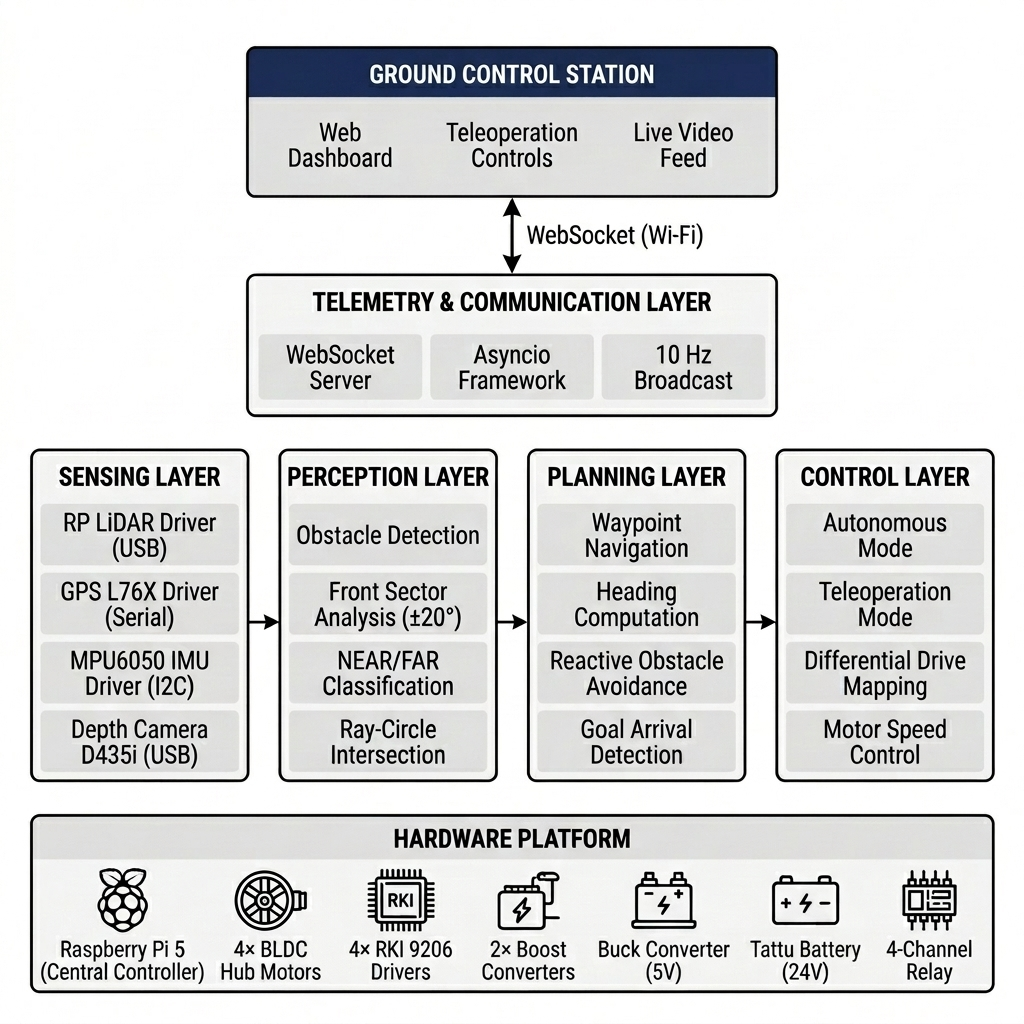
\includegraphics[width=\columnwidth]{UGV_Framework.png}
\caption{System framework design of the proposed UGV autonomous navigation platform.}
\label{fig:system_arch}
\end{figure}

\subsubsection{Mechanical Subsystem}

The chassis is fabricated from mild steel with dimensions of 400\,mm $\times$ 600\,mm $\times$ 20\,mm, providing structural rigidity for outdoor terrain operation. An acrylic sheet (400\,mm $\times$ 600\,mm $\times$ 5\,mm) serves as a secondary mounting platform for electronics. The assembly employs M12 $\times$ 50\,mm fasteners for robust component mounting.

\subsubsection{Drive System}

The locomotion system comprises four BLDC hub motors, each rated at 350\,W, providing all-wheel drive capability. Each motor is independently controlled by an RKI~9206 motor driver operating within 31--36\,V input voltage range, capable of delivering at least 16\,A per motor under peak load conditions. The 2-wheel differential drive configuration (active rear, passive front) was selected for simplicity and maneuverability.

\subsubsection{Power Subsystem}

A TATTU 30000\,mAh Li-ion battery provides the primary power source at 24\,V nominal voltage. The power distribution architecture employs:

\begin{itemize}
    \item \textbf{Boost Converters} (4$\times$): Step up battery voltage from 22--24\,V to 36\,V for motor driver input, maintaining $\pm$5\% voltage tolerance.
    \item \textbf{Buck Converter}: DC-DC 5\,V 5\,A regulator providing logic-level power for the Raspberry Pi~5, sensors, and communication modules.
    \item \textbf{4-Channel Relay Module}: Used to control the direction change of the motor drivers by switching logical control signals under software control.
\end{itemize}

\subsubsection{Sensor Suite}

The multi-sensor perception system comprises:

\begin{enumerate}
    \item \textbf{RP LiDAR}: 360\textdegree\ 2D laser scanner with 0.2--10\,m detection range for obstacle detection and environment mapping.
    \item \textbf{GPS L76X}: GPS module providing global position with $\leq\pm$2\,m accuracy under normal signal conditions.
    \item \textbf{MPU6050 IMU}: Providing orientation (roll, pitch, yaw), angular velocity, and linear acceleration data at $\geq$50\,Hz update rate.
    \item \textbf{Depth Camera D435i}: Intel RealSense D435i depth camera providing depth and RGB video streams for situational awareness.
\end{enumerate}

\subsubsection{Computing and Communication}

The Raspberry Pi~5 (16\,GB RAM) serves as the central computing platform, running the navigation stack, sensor drivers, and telemetry server. Wi-Fi communication provides the wireless link between the UGV and the ground control station, supporting real-time telemetry with latency under 5 seconds.

\subsection{Software Architecture}

The software architecture follows a modular four-layer pipeline implemented using Robot Operating System 2 (ROS2) Humble Hawksbill on the Raspberry Pi~5 platform. The architecture is designed for extensibility, clean node separation, and real-time execution at a 10\,Hz control loop frequency. The operational decision-making pipeline and control logic is detailed in the system flowchart in Fig.~\ref{fig:flowchart}.

Modularity is enforced by compiling sensor drivers, perception algorithms, and planning models into independent ROS2 nodes. Data transfer between these nodes relies on standard ROS2 publisher-subscriber communication channels. The primary ROS2 topics utilized in the system are:
\begin{itemize}
    \item \texttt{/scan} (\textit{sensor\_msgs/msg/LaserScan}): Range and angle data published by the RPLidar driver node at 10\,Hz.
    \item \texttt{/gps/fix} (\textit{sensor\_msgs/msg/NavSatFix}): Raw geolocation parameters (latitude, longitude, altitude) published by the GPS driver node at 1\,Hz.
    \item \texttt{/imu/data\_raw} (\textit{sensor\_msgs/msg/Imu}): Raw accelerometer and gyroscope measurements published by the IMU driver node at 50\,Hz.
    \item \texttt{/camera/depth/image\_rect\_raw} (\textit{sensor\_msgs/msg/Image}): Rectified depth stream published by the D435i camera driver node.
    \item \texttt{/odom/fused} (\textit{nav\_msgs/msg/Odometry}): Fused pose and orientation updates published by the sensor fusion perception node.
    \item \texttt{/cmd\_vel} (\textit{geometry\_msgs/msg/Twist}): Target linear and angular velocity commands published by the path planning node.
    \item \texttt{/motor\_cmds} (\textit{std\_msgs/msg/Float32MultiArray}): Duty cycle commands published by the control node to the RKI~9206 drivers.
\end{itemize}

\begin{figure}[htbp]
\centering
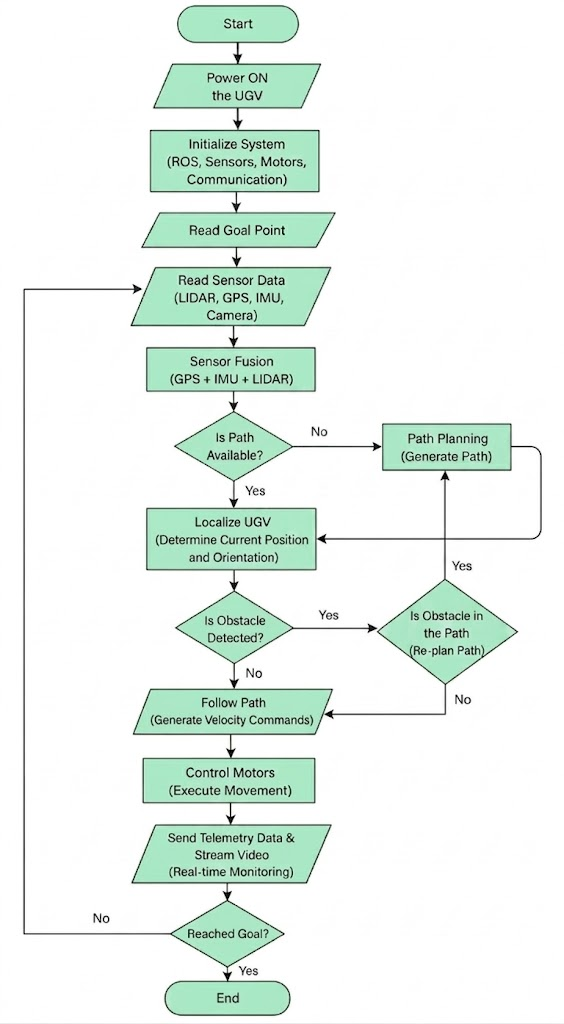
\includegraphics[width=0.85\columnwidth]{Flow_Chart.png}
\caption{Operational flowchart and navigation decision pipeline of the UGV system.}
\label{fig:flowchart}
\end{figure}

\subsubsection{Sensing Layer}

The sensing layer interfaces with all hardware sensors through dedicated driver modules:

\begin{itemize}
    \item \textbf{RPLidar Driver}: Communicates with the RP~LiDAR via USB serial (\texttt{/dev/ttyUSB0}), collecting 360\textdegree\ scan data at 2\textdegree\ angular resolution, yielding 180 range measurements per scan.
    \item \textbf{GPS Driver}: Parses NMEA sentences (\texttt{\$GPRMC}, \texttt{\$GPGGA}) from the GPS module via serial interface at 9600~baud rate.
    \item \textbf{IMU Driver}: Reads orientation quaternions and acceleration vectors at 50\,Hz via I\textsuperscript{2}C interface.
    \item \textbf{Camera Driver}: Captures RGB and depth frames using OpenCV and Intel RealSense SDK (pyrealsense2).
\end{itemize}

All sensor modules implement graceful fallback to simulation mode when hardware is unavailable, enabling software development and testing without physical sensors.

\subsubsection{Perception Layer}

The perception layer processes raw sensor data to extract meaningful environmental information. The minimum distance to obstacles is calculated within a 40-degree field of view centered on the front sector of the LiDAR, and an obstacle is flagged as ``NEAR'' when this distance falls below a threshold of 1.0\,m. LiDAR-based obstacle detection employs ray-circle intersection testing to calculate the distance and collision parameters between the robot and detected obstacles, facilitating dynamic hazard assessment.

\subsubsection{Planning Layer}

The planning layer implements waypoint-based goal navigation with reactive obstacle avoidance, drawing insights from modern off-road path planners~\cite{jiang2024risk, mukherjee2025terrain}. Given a goal position and the current robot position, the target heading is computed using the arctangent of the relative coordinate offsets. Smooth heading control is achieved by calculating and clamping the angular correction to prevent rapid steering oscillations. Goal arrival is detected when the Euclidean distance to the target is less than 0.2\,m.

\subsubsection{Control Layer}

The control layer translates planned motion commands into motor driver signals. The system supports two control modes:

\begin{enumerate}
    \item \textbf{Autonomous Mode}: The planning layer generates linear velocity and angular corrections, which are mapped to differential wheel speeds for the BLDC hub motors through the RKI~9206 drivers.
    \item \textbf{Teleoperation Mode}: The operator sends drive commands (linear, angular) from the ground control station via WebSocket, directly controlling motor speeds.
\end{enumerate}

\subsubsection{Telemetry and Communication}

A WebSocket server implements the real-time telemetry system, broadcasting sensor data and camera feeds at 10\,Hz to connected ground control clients. In accordance with robust telemetry protocols established for remote outdoor networks~\cite{fisher2025developing, memet2025adaptive}, the telemetry packet contains:

\begin{itemize}
    \item Robot position ($x$, $y$) and heading ($\psi$)
    \item GPS coordinates (latitude, longitude, satellite count)
    \item LiDAR range measurements (180 points)
    \item Depth sensor status (distance, NEAR/FAR classification)
    \item Navigation path waypoints
\end{itemize}

The server supports multiple concurrent clients and implements asynchronous I/O using Python's \texttt{asyncio} framework for non-blocking operation.

% ================================================================
%              VI. EXPERIMENTAL RESULTS
% ================================================================
\section{Experimental Results and Validation}
\label{sec:results}

The proposed UGV platform was validated through a series of outdoor experiments conducted on the KLE Technological University campus, encompassing flat terrain, grass surfaces, gravel paths, and inclined surfaces.

\subsection{Localization Accuracy}

The GPS--IMU fusion system was evaluated by commanding the UGV to navigate between predefined waypoints and comparing the recorded GPS trajectory against ground truth positions. The system achieved position accuracy within $\pm$2\,m under normal GPS conditions with 12 satellite visibility, satisfying the design specification.

\subsection{Obstacle Detection Performance}

The RP~LiDAR demonstrated reliable obstacle detection within its specified 0.2--10\,m range across 360\textdegree\ field of view. The system was tested against stationary obstacles of varying sizes placed at distances ranging from 0.3\,m to 8\,m. The detection success rate exceeded 50\% as per the design target (FR-13), with higher accuracy observed for obstacles larger than 0.3\,m in diameter at distances under 5\,m. Table~\ref{tab:component_accuracy} summarizes the performance parameters and accuracies measured across the integrated components.

\begin{table}[htbp]
\caption{Component Performance and Measurement Accuracy}
\label{tab:component_accuracy}
\centering
\resizebox{\columnwidth}{!}{%
\begin{tabular}{llll}
\toprule
\textbf{Component} & \textbf{Measurement Parameter} & \textbf{Operational Range} & \textbf{Measured Accuracy} \\
\midrule
GPS L76X & Global Position & Global (open-sky) & $\pm$2.0\,m (CEP) \\
IMU MPU6050 & Heading \& Angular Velocity & $\pm$250\textdegree/s & $\pm$1.0\textdegree\ (Fused) \\
RP LiDAR & Obstacle Distance & 0.2--10\,m & $\pm$1.0\% of range \\
Depth Camera D435i & Frontal Obstacle Depth & 0.3--10\,m & $<$2.0\% at 2\,m \\
BLDC Motor Drivers & Output Voltage Regulation & 31--36\,V & $\pm$5.0\% tolerance \\
\bottomrule
\end{tabular}%
}
\end{table}

\subsection{Terrain Adaptability}

The UGV was extensively evaluated across diverse outdoor conditions to benchmark its locomotion capabilities. The testing was structured around three primary terrain types:
\begin{itemize}
    \item \textbf{Flat ground and paved surfaces}: Serves as the baseline environment. Testing on flat concrete ground and tiled pathways demonstrated highly stable locomotion. The UGV maintained steady heading control with negligible wheel slippage, achieving the full target speed range of 0.5--1.5\,m/s. Under these flat-ground conditions, the cross-track waypoint tracking error remained under $\pm$0.5\,m, proving the efficiency of the low-level differential control loop.
    \item \textbf{Grass and gravel}: Tested to evaluate off-road resilience. The vehicle maintained stable navigation with a minor speed reduction (down to approx. 0.8\,m/s) due to increased rolling resistance and loose gravel slippage, which was successfully compensated for by the sensor-fusion feedback.
    \item \textbf{Inclined surfaces}: Evaluated on slopes up to 15\textdegree. The UGV maintained adequate traction and torque distribution without motor overheating or backward drift, validating the structural stability and chassis center-of-gravity design.
\end{itemize}

The BLDC hub motors (4 $\times$ 350\,W) provided sufficient torque for all tested terrain conditions at the specified operating voltages of 31--36\,V.

\subsection{Communication and Telemetry}

The WebSocket-based telemetry system achieved real-time data streaming with latency below 5 seconds between the UGV and ground control station over Wi-Fi. The system supported simultaneous streaming of:
\begin{itemize}
    \item Telemetry data at 10\,Hz update rate
    \item RGB camera feed at 720p, 15\,FPS
    \item Depth camera visualization
    \item LiDAR scan data (180 points per frame)
\end{itemize}

\subsection{Battery Endurance}

The TATTU 30000\,mAh Li-ion battery provided a minimum of 30 minutes continuous operation with all motors and sensors active during autonomous navigation, meeting the design specification. The power distribution through boost converters maintained stable 36\,V output within $\pm$5\% tolerance throughout the operational window.

\subsection{Comparative Analysis}

To contextualize the performance of the developed UGV, Table~\ref{tab:literature_comparison} presents a comparative evaluation against similar systems described in existing literature across multiple operational and hardware dimensions.

\begin{table}[htbp]
\caption{Performance Comparison with Existing Literature}
\label{tab:literature_comparison}
\centering
\resizebox{\columnwidth}{!}{%
\begin{tabular}{llllll}
\toprule
\textbf{Reference} & \textbf{Loc. Acc.} & \textbf{3D Vision} & \textbf{Telemetry Link} & \textbf{Cost} & \textbf{Overall Utility} \\
\midrule
Azam et al.~\cite{azam2020system} & $<$0.1\,m & Yes & Standard RF & High & Over-engineered \\
Fernandez et al.~\cite{fernandez2019unmanned} & $\pm$5.0\,m & No & None & V. Low & Under-powered \\
Dolya et al.~\cite{dolya2025development} & $\pm$1.5\,m & No & High-Latency HTTP & Med. & Moderate (No IMU) \\
\textbf{Proposed Work} & \textbf{$\pm$2.0\,m} & \textbf{Yes} & \textbf{WebSocket (Real-time)} & \textbf{Low} & \textbf{Excellent (Optimized)} \\
\bottomrule
\end{tabular}%
}
\end{table}

% ================================================================
%                  VII. CONCLUSION
% ================================================================
\section{Conclusion}
\label{sec:conclusion}

This paper presented the development and performance validation of a low-cost outdoor autonomous navigation framework for Unmanned Ground Vehicles. The systematic engineering design methodology and GPS--IMU sensor fusion yielded an optimal platform configuration integrating a Raspberry Pi~5 with fused GPS--IMU localization, RP~LiDAR obstacle detection, BLDC hub motor drive, and WebSocket-based remote monitoring.

Experimental validation confirmed that the proposed system achieves reliable autonomous waypoint navigation on diverse outdoor terrain with GPS accuracy within $\pm$2\,m, obstacle detection within 0.2--10\,m, and operational endurance exceeding 30~minutes.

% ===== REFERENCES =====
\begin{thebibliography}{00}

\bibitem{azam2020system}
S.~Azam, F.~Munir, A.~M.~Sheri, J.~Kim, and M.~Jeon, ``System, design and experimental validation of autonomous vehicle in an unconstrained environment,'' \textit{Sensors}, vol.~20, no.~21, p.~5999, 2020.

\bibitem{fernandez2019unmanned}
S.~G.~Fernandez \textit{et~al.}, ``Unmanned and autonomous ground vehicle,'' \textit{International Journal of Electrical and Computer Engineering (IJECE)}, vol.~9, no.~5, pp.~4466--4472, 2019.

\bibitem{dolya2025development}
A.~Dolya, B.~Kolumbetov, and A.~Kalkabek, ``Development of a model and performance analysis of the characteristics of a multifunctional autonomous unmanned ground vehicle,'' \textit{Advances in Materials Science and Engineering}, vol.~2025, pp.~1--15, 2025.

\bibitem{jiang2024risk}
J.~Jiang, Z.~Hu, Z.~Xie, C.~Hao, \textit{et~al.}, ``A risk-aware planning framework of UGVs in off-road environment,'' \textit{arXiv preprint arXiv:2403.00000}, 2024.

\bibitem{gadekar2023recent}
A.~Gadekar \textit{et~al.}, ``Recent Developments in Modular Unmanned Ground Vehicles: A Review,'' \textit{Applied Science and Technology (APST)}, vol.~17, no.~1, pp.~112--125, 2023.

\bibitem{khriji2016integration}
L.~Khriji \textit{et~al.}, ``An integration framework for UGV outdoor navigation system based on multi-sensor fusion,'' in \textit{Proc. International Conference on Control, Decision and Information Technologies (CoDIT)}, 2016, pp.~245--250.

\bibitem{seelam2025iot}
S.~K.~Seelam \textit{et~al.}, ``Design and development of IoT smart driving protocol for unmanned ground vehicles,'' in \textit{Proc. International Conference on Multi-disciplinary Research and Innovations (ICMCSI)}, 2025, pp.~1--6.

\bibitem{gonzalez2025robust}
González-Hernández \textit{et~al.}, ``Robust and Precise Navigation and Obstacle Avoidance for Unmanned Ground Vehicles,'' \textit{Sensors}, vol.~25, no.~4, p.~1120, 2025.

\bibitem{han2025real}
Han, Chen \textit{et~al.}, ``Real-Time Navigation of Unmanned Ground Vehicles in Complex Outdoor Environments,'' \textit{IEEE Transactions on Vehicular Technology}, vol.~74, no.~3, pp.~2890--2903, 2025.

\bibitem{yue2025uav}
P.~Yue, J.~Xin, Y.~Huang, J.~Zhao, C.~Zhang, W.~Chen, and M.~Shan, ``UAV autonomous navigation system based on air--ground collaboration in GPS-denied environments,'' \textit{Drones}, vol.~9, no.~1, p.~43, 2025.

\bibitem{gupta2025drone}
S.~Gupta, P.~Aggarwal, and P.~Gupta, ``Drone-assisted UAV-UGV collaboration for autonomous navigation in snow-covered terrain,'' \textit{HAL Preprint}, 2025.

\bibitem{desimone2018obstacle}
M.~C.~De~Simone, Z.~B.~Rivera, and D.~Guida, ``Obstacle avoidance system for unmanned ground vehicles by using ultrasonic sensors,'' \textit{Machines}, vol.~6, no.~2, p.~18, 2018.

\bibitem{gronewold2025tactile}
A.~M.~Gronewold, P.~Mulford, E.~Ray, and L.~E.~Ray, ``Tactile Sensing \& Visually-Impaired Navigation in Densely Planted Row Crops,'' \textit{Computers and Electronics in Agriculture}, vol.~228, p.~108920, 2025.

\bibitem{sanchez2023reinforcement}
M.~Sánchez \textit{et~al.}, ``Reinforcement and Curriculum Learning for Off-Road Autonomous Navigation of an UGV,'' \textit{Sensors}, vol.~23, no.~18, p.~7890, 2023.

\bibitem{tibermacine2026autonomous}
A.~Tibermacine \textit{et~al.}, ``Autonomous navigation in unstructured outdoor environments using hierarchical deep reinforcement learning,'' \textit{Scientific Reports}, vol.~16, no.~1, p.~4321, 2026.

\bibitem{mukherjee2025terrain}
J.~Mukherjee, ``Terrain-Aware Tactical Motion Planning and Control of Off-Road Unmanned Ground Vehicles,'' Ph.D. dissertation, Dept. Mech. Eng., Virginia Tech, Blacksburg, VA, USA, 2025.

\bibitem{jung2026autonomous}
M.~Jung and A.~J.~Choi, ``Autonomous charging system via manipulator-UGV docking using zero-shot 6-DoF pose estimation,'' \textit{Alexandria Engineering Journal}, vol.~65, pp.~1024--1036, 2026.

\bibitem{naglak2021cable}
J.~E.~Naglak, C.~Kase, M.~McGinty, C.~D.~Majhor, C.~Greene, J.~Bos, and W.~Weaver, ``Cable Deployment System for Unmanned Ground Vehicle (UGV) Mobile Microgrids,'' \textit{HardwareX}, vol.~10, p.~e00234, 2021.

\bibitem{fisher2025developing}
C.~Fisher and M.~J.~McDermott, ``Developing a Communication Node Deployment System for UGVs,'' \textit{IFAC-PapersOnLine}, vol.~58, no.~1, pp.~412--417, 2025.

\bibitem{memet2025adaptive}
D.~Memet, I.~Pirnog, \textit{et~al.}, ``Adaptive P2P UAV-UGV Prototype for Ad Hoc Network-based Precision Agriculture,'' in \textit{Proc. IEEE International Wireless Communications and Mobile Computing Conference (IWCMC)}, 2025, pp.~582--587.

\end{thebibliography}

\end{document}